\usetikzlibrary{fit,arrows}

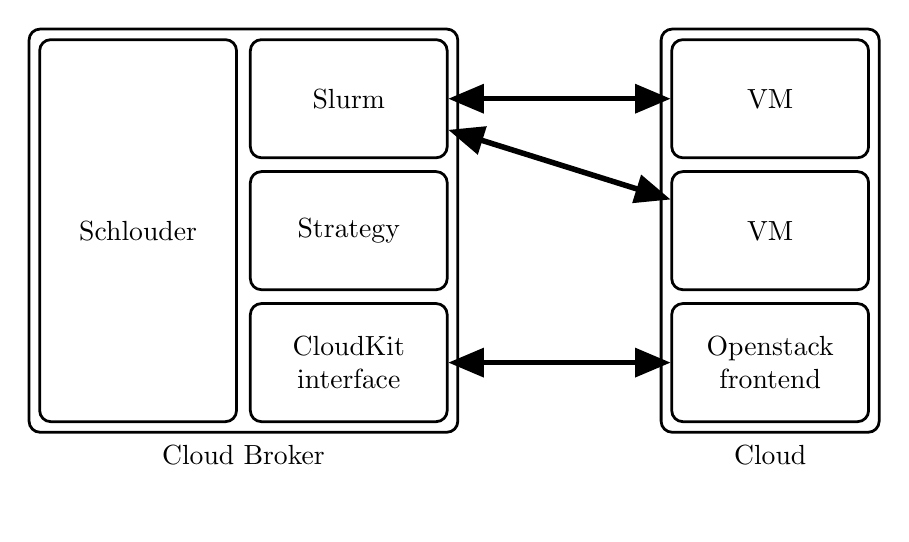
\begin{tikzpicture}[node distance=5pt,x=25mm+5pt,y=15mm+5pt,
every node/.style={anchor=center,
line width=1pt,
minimum width = 25mm,
minimum height =15mm,
rounded corners,
label distance=-5mm,
draw 
},
high/.style={%
minimum height =45mm+10pt,
},
large/.style={%
minimum width=50mm+5pt
}]
\node[high]at(0,0)(app){Schlouder};
\node[align=center]at(1,-1)(ck){CloudKit\\interface};
\node[]at(1,0)(strat){Strategy};
\node[]at(1,1)(slm){Slurm};
\node[align=center]at(3,-1)(cc){Openstack\\frontend};
\node[]at(3,0)(vm1){VM};
\node[]at(3,1)(vm2){VM};
\node[draw,fit=(app)(ck)(slm),label={below:Cloud Broker}]{};
\node[draw,fit=(vm2)(cc)(vm1),label={below:Cloud}]{};
\draw [{triangle 45}-{triangle 45},line width=2pt] (ck)--(cc);
\draw [{triangle 45}-{triangle 45},line width=2pt] (vm2)--(slm);
\draw [{triangle 45}-{triangle 45},line width=2pt] (vm1)--(slm);
%\draw [{triangle 45}-{triangle 45},shorten <=10pt,shorten >=10pt] (1,0)--(1,1);
%\draw [{triangle 45}-{triangle 45},shorten <=10pt,shorten >=10pt] (1,0)--(1,-1);
\end{tikzpicture}
